%%%%%%%%%%%%%%%%%%%%%%%%%%%%%%%%%%%%%%%%%%%%%%%%%%%%%%%%%%%%%%%%%%%%%%%
% BAB 3
%%%%%%%%%%%%%%%%%%%%%%%%%%%%%%%%%%%%%%%%%%%%%%%%%%%%%%%%%%%%%%%%%%%%%%%

\mychapter{4}{BAB 4 METODOLOGI}

\section{Tahapan Pelaksanaan}

Pelaksanaan Praktik Kerja Lapang (PKL) pada pengembangan aplikasi web SIPANTAU dilakukan dengan melanjutkan pengembangan sistem yang telah berjalan sebelumnya. Pada awal pelaksanaan PKL, sistem telah memiliki antarmuka \textit{frontend} yang menggunakan data \textit{dummy}, rancangan awal basis data, serta kebutuhan utama sistem yang meliputi pengelolaan data komoditas, prediksi harga komoditas untuk tiga hari ke depan pada pasar tertentu, dan penerapan autentikasi serta otorisasi berdasarkan peran pengguna. Selain itu, Laravel telah ditetapkan sebagai \textit{framework} yang digunakan pada sisi \textit{backend}. Kondisi tersebut menjadi dasar dalam melakukan analisis terhadap sistem yang telah tersedia serta menentukan komponen yang perlu dirancang dan dikembangkan selama pelaksanaan PKL. Dengan demikian, kegiatan pengembangan difokuskan pada basis data dan \textit{backend}, mekanisme autentikasi dan otorisasi, integrasi layanan model prediksi, serta \textit{deployment} aplikasi.

Tahapan pelaksanaan diawali dengan analisis kondisi dan kebutuhan sistem yang telah ada untuk memahami kebutuhan fungsional serta hubungan antara \textit{frontend}, \textit{backend}, basis data, dan layanan model prediksi. Berdasarkan hasil analisis tersebut, dilakukan perancangan basis data dan arsitektur \textit{backend}, perancangan autentikasi dan otorisasi, perancangan integrasi layanan model prediksi, serta perancangan \textit{deployment} aplikasi. Setiap rancangan kemudian menjadi dasar bagi tahap implementasi masing-masing komponen. Implementasi dilakukan secara bertahap mulai dari basis data dan \textit{backend}, kemudian autentikasi dan otorisasi, integrasi layanan model prediksi, hingga \textit{deployment} aplikasi.

\begin{figure}[H]
    \centering
    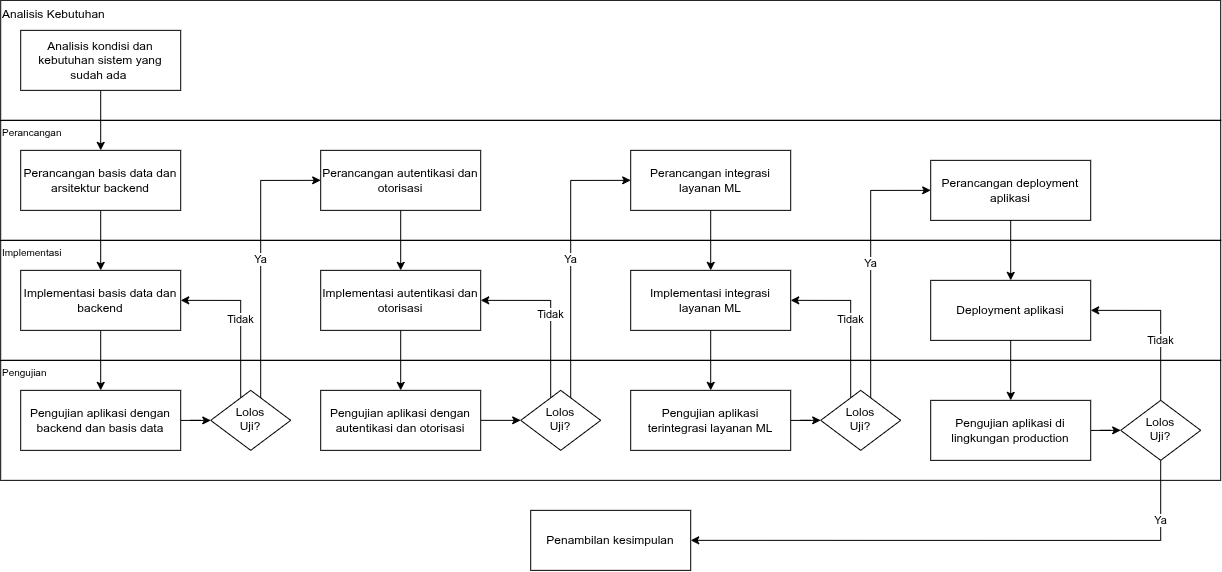
\includegraphics[width=\textwidth]{img/tahapan-pelaksanaan.png}
    \caption{Tahapan Pelaksanaan PKL}
    \label{fig:tahapan-pelaksanaan}
\end{figure}

Setiap hasil implementasi diuji sebelum proses dilanjutkan ke tahap berikutnya. Apabila hasil pengujian belum memenuhi kebutuhan yang ditetapkan, dilakukan penyesuaian terhadap implementasi terkait dan pengujian dilakukan kembali hingga hasil yang diperoleh sesuai dengan kebutuhan sistem. Setelah seluruh komponen aplikasi berhasil melalui pengujian pada lingkungan pengembangan, dilakukan \textit{deployment} ke lingkungan \textit{production} yang telah dirancang. Aplikasi yang telah di-\textit{deploy} kemudian diuji kembali pada lingkungan \textit{production} untuk memastikan sistem dapat berjalan pada lingkungan operasional. Tahapan pelaksanaan secara keseluruhan ditunjukkan pada Gambar~\ref{fig:tahapan-pelaksanaan}.

\section{Spesifikasi Hardware dan Software}

Pengembangan dan \textit{deployment} aplikasi web SIPANTAU dilakukan pada lingkungan komputasi berbasis \textit{Virtual Private Server} (VPS). Infrastruktur tersebut menggunakan virtualisasi Xen dengan arsitektur x86-64 dan sistem operasi Ubuntu 24.04.4 LTS. Server menyediakan 8 \textit{virtual CPU} dengan prosesor Intel Xeon E5-2620 v4 berfrekuensi 2.10 GHz serta memori sebesar 4 GB. Spesifikasi perangkat keras tersebut digunakan sebagai lingkungan untuk menjalankan komponen aplikasi selama proses pengembangan dan \textit{deployment}. Rincian spesifikasi perangkat keras yang digunakan ditunjukkan pada Tabel~\ref{tab:spesifikasi-hardware}.

\begin{table}[H]
    \centering
    \caption{Spesifikasi Perangkat Keras}
    \label{tab:spesifikasi-hardware}
    \begin{tabular}{|l|l|}
        \hline
        \textbf{Komponen} & \textbf{Spesifikasi} \\ \hline
        Jenis perangkat & Virtual Private Server (VPS) \\ \hline
        Virtualisasi & Xen \\ \hline
        Prosesor & Intel Xeon E5-2620 v4 @ 2.10 GHz \\ \hline
        CPU & 8 vCPU \\ \hline
        Memori & 4 GB \\ \hline
        Arsitektur & x86-64 \\ \hline
        Sistem operasi & Ubuntu 24.04.4 LTS \\ \hline
    \end{tabular}
\end{table}

Perangkat lunak yang digunakan terdiri atas komponen untuk pengembangan \textit{backend}, pengelolaan basis data, pengembangan \textit{frontend}, penyajian aplikasi, serta pengelolaan lingkungan aplikasi. Laravel 12.49.0 digunakan sebagai \textit{framework backend} dengan PHP 8.4.21 sebagai lingkungan eksekusinya, sedangkan Composer 2.9.8 digunakan untuk mengelola dependensi PHP. Basis data aplikasi menggunakan MySQL 8.4.8, sementara sisi \textit{frontend} menggunakan Node.js 20.20.2 dan NPM 10.8.2 sebagai lingkungan dan pengelola paket JavaScript. Docker 29.4.0 digunakan untuk menjalankan komponen aplikasi dalam lingkungan \textit{container}, Nginx 1.29.8 digunakan sebagai \textit{web server}, dan Git 2.43.0 digunakan untuk pengelolaan versi kode sumber. Rincian perangkat lunak yang digunakan ditunjukkan pada Tabel~\ref{tab:spesifikasi-software}.

\begin{table}[H]
    \centering
    \caption{Spesifikasi Perangkat Lunak}
    \label{tab:spesifikasi-software}
    \begin{tabular}{|l|l|l|}
        \hline
        \textbf{Perangkat Lunak} & \textbf{Versi} & \textbf{Fungsi} \\ \hline
        Ubuntu & 24.04.4 LTS & Sistem operasi \\ \hline
        PHP & 8.4.21 & Runtime backend \\ \hline
        Laravel & 12.49.0 & Framework backend \\ \hline
        Composer & 2.9.8 & Pengelola dependensi PHP \\ \hline
        MySQL & 8.4.8 & Sistem manajemen basis data \\ \hline
        Node.js & 20.20.2 & Runtime JavaScript frontend \\ \hline
        NPM & 10.8.2 & Pengelola paket frontend \\ \hline
        Nginx & 1.29.8 & Web server \\ \hline
        Docker & 29.4.0 & Pengelola container \\ \hline
        Git & 2.43.0 & Version control \\ \hline
    \end{tabular}
\end{table}

\section{Metode Perancangan}

Metode perancangan digunakan sebagai dasar dalam menentukan struktur dan mekanisme kerja komponen aplikasi yang akan dikembangkan sebelum dilakukan implementasi. Perancangan dilakukan berdasarkan kondisi awal sistem, kebutuhan aplikasi, serta keterkaitan antara komponen yang telah tersedia dengan komponen yang perlu dikembangkan. Proses perancangan mencakup basis data dan arsitektur \textit{backend}, mekanisme \textit{authentication} dan \textit{authorization}, integrasi layanan model prediksi, serta \textit{deployment} aplikasi. Setiap rancangan disusun untuk menghasilkan spesifikasi teknis yang dapat digunakan sebagai acuan pada tahap implementasi.

\subsection{Analisis Kondisi dan Kebutuhan Sistem}

Analisis kondisi dan kebutuhan sistem dilakukan untuk memahami keadaan awal aplikasi serta menentukan fungsi yang perlu disediakan oleh komponen yang dikembangkan. Pada awal pelaksanaan PKL, aplikasi telah memiliki \textit{frontend} yang menggunakan data \textit{dummy}, rancangan awal basis data, dan kebutuhan utama sistem. Kebutuhan tersebut mencakup pengelolaan data komoditas, prediksi harga komoditas untuk tiga hari ke depan pada pasar tertentu, serta penerapan \textit{authentication} dan \textit{authorization} berdasarkan peran pengguna. Selain kebutuhan tersebut, Laravel telah ditetapkan sebagai \textit{framework} yang digunakan untuk membangun sisi \textit{backend}. Hasil analisis terhadap kondisi dan kebutuhan tersebut kemudian digunakan sebagai dasar untuk menentukan rancangan basis data, arsitektur \textit{backend}, mekanisme pengendalian akses, integrasi layanan model prediksi, dan kebutuhan \textit{deployment}.

\subsection{Perancangan Basis Data dan Arsitektur Backend}

Perancangan basis data dilakukan dengan menyesuaikan struktur penyimpanan data terhadap kebutuhan fungsional aplikasi. Proses perancangan mencakup penentuan entitas yang diperlukan, atribut pada setiap entitas, serta hubungan antarentitas yang digunakan dalam pengelolaan data aplikasi. Hasil perancangan basis data digunakan sebagai acuan dalam menentukan struktur tabel dan relasi yang akan diimplementasikan pada sistem manajemen basis data. Rancangan basis data kemudian diselaraskan dengan kebutuhan \textit{backend} agar data yang diperlukan oleh setiap fungsi aplikasi dapat disediakan secara terstruktur.

Perancangan arsitektur \textit{backend} dilakukan untuk menentukan pembagian komponen dan aliran data antara \textit{frontend}, \textit{backend}, basis data, dan layanan pendukung lainnya. Laravel digunakan sebagai dasar perancangan sisi \textit{backend}, dengan komponen aplikasi disusun berdasarkan tanggung jawab masing-masing dalam menerima permintaan, memproses data, berinteraksi dengan basis data, dan menghasilkan respons kepada \textit{frontend}. Perancangan juga mencakup penentuan \textit{route} dan mekanisme komunikasi yang diperlukan agar fungsi pengelolaan data dan fungsi lainnya dapat diakses oleh \textit{frontend}. Rancangan tersebut selanjutnya digunakan sebagai acuan pada tahap implementasi \textit{backend} dan basis data.

\subsection{Perancangan Authentication dan Authorization}

Perancangan \textit{authentication} dan \textit{authorization} dilakukan untuk memastikan bahwa akses terhadap fungsi dan sumber daya aplikasi diberikan sesuai dengan identitas serta peran pengguna. Mekanisme \textit{authentication} dirancang untuk melakukan verifikasi terhadap pengguna sebelum pengguna dapat mengakses fungsi yang memerlukan autentikasi. Setelah pengguna berhasil diautentikasi, sistem menggunakan informasi peran pengguna sebagai dasar dalam menentukan hak akses terhadap sumber daya dan fungsi tertentu. Dengan demikian, pengguna dengan peran yang berbeda dapat memiliki tingkat akses yang berbeda sesuai dengan kebutuhan sistem.

Perancangan hak akses dilakukan menggunakan pendekatan berbasis peran, dengan setiap peran memiliki kumpulan izin terhadap fungsi atau sumber daya tertentu. Hubungan antara pengguna, peran, dan hak akses ditentukan terlebih dahulu agar mekanisme pengendalian akses dapat diterapkan secara konsisten pada \textit{backend}. Rancangan tersebut kemudian menjadi dasar dalam menentukan mekanisme pemeriksaan hak akses pada setiap fungsi atau \textit{endpoint} yang membutuhkan pembatasan akses. Hasil perancangan ini selanjutnya digunakan sebagai acuan dalam implementasi \textit{authentication} dan \textit{authorization}.

\subsection{Perancangan Integrasi Layanan Model Prediksi}

Perancangan integrasi layanan model prediksi dilakukan untuk menentukan mekanisme pertukaran data antara aplikasi web dengan model prediksi yang telah tersedia. Model prediksi tidak dikembangkan atau dilatih kembali dalam pelaksanaan PKL, melainkan digunakan sebagai komponen yang diintegrasikan ke dalam aplikasi untuk menghasilkan prediksi harga komoditas. Perancangan difokuskan pada aliran data mulai dari permintaan prediksi oleh pengguna, pengambilan data historis yang diperlukan, persiapan data, pemanggilan model, hingga pengembalian hasil prediksi kepada \textit{frontend}. Alur tersebut dirancang agar proses prediksi dapat dijalankan melalui aplikasi tanpa mengharuskan pengguna berinteraksi secara langsung dengan model.

Data yang digunakan sebagai masukan model perlu dipersiapkan dalam format yang sesuai dengan kebutuhan layanan prediksi. Oleh karena itu, rancangan integrasi mencakup proses pengambilan data historis komoditas dari basis data, penyesuaian struktur data, pengiriman data kepada pipeline model prediksi, serta pengolahan hasil prediksi sebelum diberikan kepada \textit{frontend}. Pipeline Chronos-v2 digunakan sebagai komponen prediksi dalam rancangan tersebut. Secara umum, aliran integrasi dirancang dari \textit{frontend} menuju \textit{backend}, kemudian menuju pipeline model prediksi, dan hasil prediksi dikembalikan melalui \textit{backend} untuk ditampilkan kepada pengguna.

\subsection{Perancangan Deployment Aplikasi}

Perancangan \textit{deployment} dilakukan untuk menentukan konfigurasi lingkungan yang diperlukan agar aplikasi dapat dijalankan pada lingkungan \textit{production}. Perancangan mencakup pembagian komponen aplikasi ke dalam lingkungan eksekusi, konfigurasi layanan aplikasi, koneksi basis data, serta komunikasi antara \textit{frontend}, \textit{backend}, dan layanan pendukung. Penggunaan Docker dirancang untuk menyediakan lingkungan eksekusi berbasis \textit{container} bagi komponen aplikasi, sedangkan Nginx digunakan sebagai bagian dari konfigurasi penyajian aplikasi. Rancangan tersebut juga mempertimbangkan konfigurasi variabel lingkungan dan dependensi yang diperlukan oleh masing-masing komponen.

Rancangan \textit{deployment} digunakan sebagai acuan dalam proses pemasangan dan konfigurasi aplikasi pada VPS. Setelah aplikasi berhasil ditempatkan pada lingkungan \textit{production}, dilakukan pengujian untuk memastikan setiap komponen dapat berkomunikasi dan menjalankan fungsi sesuai dengan rancangan. Apabila ditemukan permasalahan pada hasil pengujian, konfigurasi atau komponen \textit{deployment} disesuaikan dan proses \textit{deployment} serta pengujian dilakukan kembali. Dengan demikian, rancangan \textit{deployment} tidak hanya menentukan konfigurasi awal lingkungan \textit{production}, tetapi juga menjadi dasar dalam proses penyesuaian hingga aplikasi dapat berjalan sesuai kebutuhan.

\section{Metode Implementasi}

Metode implementasi merupakan tahapan penerapan hasil perancangan menjadi komponen aplikasi yang dapat dijalankan dan digunakan sesuai dengan kebutuhan sistem. Implementasi dilakukan secara bertahap berdasarkan rancangan basis data dan arsitektur \textit{backend}, mekanisme \textit{authentication} dan \textit{authorization}, integrasi layanan model prediksi, serta rancangan \textit{deployment}. Setiap komponen diimplementasikan sesuai dengan rancangan yang telah ditetapkan dan disesuaikan apabila ditemukan kondisi teknis yang memerlukan perubahan selama proses pengembangan. Hasil implementasi pada setiap tahapan selanjutnya digunakan sebagai dasar untuk melakukan pengujian terhadap fungsi yang telah dikembangkan.

\subsection{Implementasi Basis Data dan Backend}

Implementasi basis data dilakukan dengan merealisasikan rancangan struktur data ke dalam MySQL menggunakan mekanisme migration Laravel. Migration digunakan untuk membentuk tabel, atribut, serta relasi yang diperlukan oleh aplikasi sesuai dengan kebutuhan sistem. Selain itu, data awal yang diperlukan oleh aplikasi dimasukkan menggunakan mekanisme seeder yang tersedia pada Laravel. Struktur basis data yang telah dibuat kemudian digunakan oleh \textit{backend} sebagai sumber data dalam menjalankan fungsi pengelolaan data aplikasi.

Implementasi \textit{backend} dilakukan menggunakan Laravel dengan menerapkan pola \textit{Model} dan \textit{Controller} untuk menangani interaksi antara aplikasi dan basis data. Controller digunakan untuk menerima permintaan dari \textit{frontend}, melakukan pemrosesan yang diperlukan, serta menghasilkan respons melalui \textit{API}. Fungsi pengelolaan data diimplementasikan melalui beberapa Controller yang menangani data komoditas, pasar, panen, harga pasar harian, harga petani harian, dan ketersediaan harian. Data yang diperoleh dari basis data kemudian disusun menjadi respons API menggunakan komponen \textit{Resource} pada Laravel sebelum diteruskan kepada \textit{frontend}.

\subsection{Implementasi Authentication dan Authorization}

Implementasi \textit{authentication} dilakukan melalui \textit{endpoint} yang disediakan oleh AuthController. Proses tersebut mencakup pendaftaran pengguna, proses \textit{login}, pengelolaan sesi autentikasi, dan \textit{logout}. Laravel Sanctum digunakan sebagai mekanisme autentikasi berbasis token untuk mengidentifikasi pengguna yang melakukan permintaan terhadap layanan \textit{backend}. Token autentikasi kemudian digunakan dalam permintaan yang membutuhkan identitas pengguna, sehingga sistem dapat membedakan permintaan yang telah terautentikasi dengan permintaan yang tidak memiliki autentikasi yang valid.

Implementasi \textit{authorization} dilakukan dengan menerapkan pembatasan akses berdasarkan peran dan izin pengguna menggunakan paket \textit{Spatie Laravel Permission}. Peran dan izin disimpan pada basis data melalui tabel yang disediakan oleh paket tersebut, kemudian digunakan untuk menentukan fungsi yang dapat diakses oleh pengguna. Mekanisme pembatasan akses diterapkan pada \textit{endpoint} yang memerlukan hak akses tertentu sehingga pengguna hanya dapat menjalankan operasi sesuai dengan peran dan izin yang dimilikinya. Selain itu, informasi aktivitas pengguna dicatat melalui ActivityLogger pada fungsi tertentu, termasuk ketika pengguna mengakses fungsi prediksi.

\subsection{Implementasi Integrasi Layanan Model Prediksi}

Implementasi integrasi layanan model prediksi dilakukan dengan menghubungkan \textit{backend} Laravel dengan layanan model prediksi yang dijalankan secara terpisah. Ketika pengguna meminta prediksi berdasarkan komoditas dan pasar tertentu, \textit{frontend} mengirimkan pasar\_id dan komoditas\_id kepada \textit{backend}. Parameter tersebut terlebih dahulu divalidasi untuk memastikan bahwa pasar dan komoditas yang diminta tersedia pada basis data. Selanjutnya, \textit{backend} mengambil data harga pasar harian dan data pendukung berupa ketersediaan, kebutuhan, serta neraca harian berdasarkan komoditas dan pasar yang dipilih. Data yang digunakan dibatasi pada sepuluh data historis terakhir dan diurutkan kembali berdasarkan urutan waktu sebelum digunakan sebagai masukan model. Alur integrasi layanan model prediksi secara keseluruhan ditunjukkan pada Gambar \ref{fig:alur-prediksi}.

\begin{figure}[H]
    \centering
    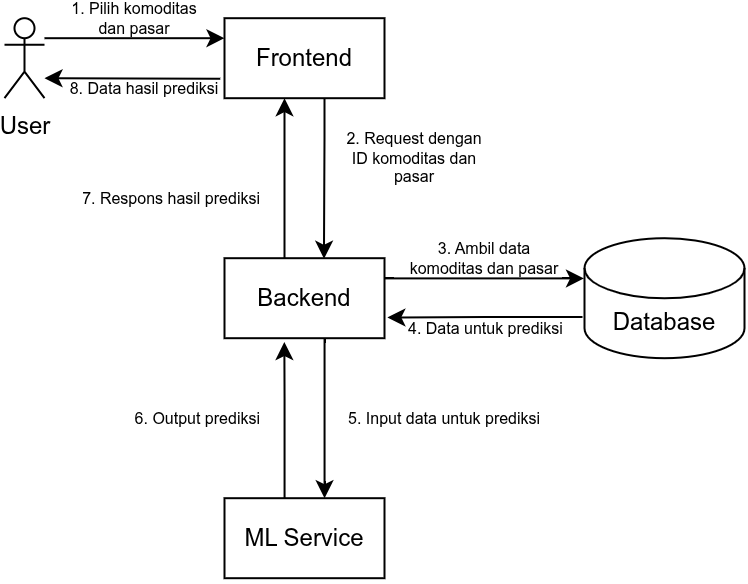
\includegraphics[width=0.8\textwidth]{img/alur-prediksi.png}
    \caption{Alur integrasi layanan model prediksi}
    \label{fig:alur-prediksi}
\end{figure}

Data historis yang telah diperoleh kemudian disusun menjadi struktur masukan yang terdiri atas nilai harga pasar, ketersediaan harian, kebutuhan harian, dan neraca harian. Setiap nilai dikonversi menjadi tipe numerik sebelum dikirimkan kepada layanan model prediksi. \textit{Backend} kemudian melakukan permintaan HTTP \textit{POST} ke layanan \textit{machine learning} pada /predict melalui jaringan internal Docker dengan alamat layanan ml-service:8001. Data tersebut dikirimkan dalam parameter data sebagai masukan untuk proses prediksi.

Layanan model prediksi diimplementasikan menggunakan FastAPI dan menyediakan \textit{endpoint} POST /predict untuk menerima data dari \textit{backend}. Data masukan dikonversi menjadi array numerik menggunakan NumPy, kemudian dilakukan transformasi dimensi agar sesuai dengan struktur masukan yang dibutuhkan oleh pipeline model. Pipeline Chronos-2 yang digunakan pada layanan tersebut dimuat menggunakan model autogluon/chronos2-small, dengan pemilihan perangkat komputasi GPU apabila tersedia dan CPU apabila GPU tidak tersedia.

Pipeline model kemudian dijalankan dengan panjang prediksi sebanyak tiga periode. Hasil prediksi yang diperoleh diproses untuk memperoleh nilai prediksi yang digunakan oleh aplikasi, kemudian dikembalikan oleh layanan model dalam bentuk respons JSON dengan atribut prediksi. \textit{Backend} Laravel menerima respons tersebut dan memetakan tiga nilai prediksi menjadi prediksi untuk hari pertama, hari kedua, dan hari ketiga. Hasil tersebut kemudian digabungkan dengan informasi tanggal dan harga pasar historis yang relevan sebelum dikembalikan kepada \textit{frontend} melalui respons API.

\subsection{Deployment Aplikasi}

Deployment aplikasi dilakukan pada VPS dengan menggunakan Docker untuk menjalankan komponen aplikasi dalam beberapa \textit{container}. Lingkungan \textit{production} terdiri atas \textit{container} backend, frontend, ml-service, dan nginx. Container backend digunakan untuk menjalankan aplikasi Laravel, sedangkan frontend menjalankan aplikasi sisi \textit{frontend}. Layanan model prediksi dijalankan pada ml-service, sementara Nginx digunakan untuk menerima akses dari luar dan meneruskan permintaan kepada komponen aplikasi yang sesuai.

Setiap komponen dihubungkan melalui jaringan Docker sipantau-network sehingga \textit{backend} dapat berkomunikasi dengan layanan model prediksi menggunakan nama layanan ml-service. Container backend, ml-service, dan frontend dikonfigurasi dengan restart unless-stopped agar layanan dapat dijalankan kembali secara otomatis apabila container berhenti dan Docker daemon tetap berjalan. Nginx mengekspos port 80 dan 443 untuk menyediakan akses HTTP dan HTTPS dari luar lingkungan Docker. Konfigurasi tersebut digunakan sebagai dasar dalam menjalankan aplikasi pada lingkungan \textit{production}.

\section{Metode Pengujian}

Metode pengujian digunakan untuk memastikan bahwa komponen aplikasi yang telah diimplementasikan dapat berjalan sesuai dengan kebutuhan dan rancangan sistem. Pengujian dilakukan secara bertahap pada setiap komponen dan dilanjutkan dengan pengujian setelah komponen tersebut terintegrasi dengan \textit{frontend}. Pengujian dilakukan terhadap basis data dan \textit{backend}, mekanisme \textit{authentication} dan \textit{authorization}, integrasi layanan model prediksi, serta aplikasi pada lingkungan \textit{production}. Pada pengujian tingkat layanan, permintaan dilakukan secara langsung terhadap \textit{endpoint} menggunakan Postman atau perintah \texttt{curl}, sedangkan pengujian integrasi dilakukan melalui antarmuka aplikasi untuk memastikan alur penggunaan oleh pengguna dapat berjalan dengan baik. Hasil dari setiap pengujian kemudian dibandingkan dengan kondisi atau keluaran yang diharapkan untuk menentukan kesesuaian implementasi terhadap kebutuhan sistem.

\subsection{Pengujian Basis Data dan Backend}

Pengujian basis data dan \textit{backend} dilakukan untuk memastikan bahwa fungsi pengelolaan data dan \textit{endpoint} API dapat menerima permintaan, memproses data, serta menghasilkan respons sesuai dengan kebutuhan sistem. Pengujian dilakukan menggunakan Postman terhadap setiap \textit{endpoint} yang disediakan oleh \textit{backend}, termasuk \textit{endpoint} untuk pengelolaan data aplikasi. Pengujian dilakukan dengan memberikan permintaan dan parameter yang sesuai dengan fungsi masing-masing \textit{endpoint}, kemudian memeriksa respons yang dihasilkan serta perubahan data pada basis data apabila operasi tersebut melakukan penyimpanan atau perubahan data. Setelah \textit{backend} diintegrasikan dengan \textit{frontend}, pengujian kembali dilakukan melalui antarmuka aplikasi untuk memastikan bahwa permintaan dari \textit{frontend} dapat diproses oleh \textit{backend} dan hasilnya dapat digunakan oleh aplikasi. Dengan demikian, pengujian tidak hanya memeriksa fungsi API secara langsung, tetapi juga memastikan keterhubungan antara \textit{frontend}, \textit{backend}, dan basis data. Ringkasan aspek pengujian, metode yang digunakan, dan hasil yang diharapkan ditunjukkan pada Tabel \ref{tab:pengujian-backend}.

\begin{longtable}{|p{3.2cm}|p{4.0cm}|p{4.0cm}|}
    \caption{Ringkasan pengujian basis data dan backend}
    \label{tab:pengujian-backend} \\
    \hline
    \textbf{Aspek Pengujian} & \textbf{Metode Pengujian} & \textbf{Hasil yang Diharapkan} \\
    \hline
    \endfirsthead

    \hline
    \textbf{Aspek Pengujian} & \textbf{Metode Pengujian} & \textbf{Hasil yang Diharapkan} \\
    \hline
    \endhead

    Endpoint API &
    Mengirimkan permintaan pada setiap endpoint menggunakan Postman &
    Endpoint dapat menerima dan memproses permintaan serta menghasilkan respons sesuai fungsi. \\
    \hline

    \hline
    Pengelolaan data &
    Melakukan operasi penambahan, pembacaan, perubahan, dan penghapusan data sesuai fungsi endpoint &
    Data pada basis data berubah sesuai dengan operasi yang dilakukan. \\
    \hline
    Integrasi frontend--backend &
    Menjalankan fungsi aplikasi melalui frontend setelah backend terintegrasi &
    Permintaan dari frontend dapat diproses oleh backend dan hasilnya dapat digunakan oleh aplikasi. \\
    \hline
\end{longtable}

\subsection{Pengujian Authentication dan Authorization}

Pengujian \textit{authentication} dan \textit{authorization} dilakukan untuk memastikan bahwa mekanisme akses pengguna berjalan sesuai dengan peran yang dimiliki. Pengujian diawali dengan membuat beberapa akun pengguna dengan peran yang berbeda, kemudian melakukan pengujian terhadap fungsi yang seharusnya dapat diakses maupun tidak dapat diakses oleh masing-masing peran. Pengujian dilakukan menggunakan Postman dengan mengirimkan permintaan menggunakan akun dari setiap peran dan mengamati respons yang diberikan oleh \textit{backend}. Setelah mekanisme tersebut diintegrasikan dengan \textit{frontend}, pengujian dilanjutkan melalui beberapa skenario penggunaan untuk memastikan bahwa pengguna dapat menjalankan fungsi yang menjadi hak aksesnya dan tidak dapat menjalankan fungsi yang berada di luar hak akses tersebut. Hasil pengujian digunakan untuk memastikan kesesuaian antara peran pengguna dan hak akses terhadap fungsi aplikasi. Rincian aspek pengujian, metode pengujian, dan hasil yang diharapkan dirangkum pada Tabel \ref{tab:pengujian-auth}.

\begin{longtable}{|p{3.2cm}|p{4.0cm}|p{4.0cm}|}
    \caption{Ringkasan pengujian authentication dan authorization}
    \label{tab:pengujian-auth} \\
    \hline
    \textbf{Aspek Pengujian} & \textbf{Metode Pengujian} & \textbf{Hasil yang Diharapkan} \\
    \hline
    \endfirsthead
    
    \hline
    \textbf{Aspek Pengujian} & \textbf{Metode Pengujian} & \textbf{Hasil yang Diharapkan} \\
    \hline
    \endhead
    
    Authentication &
    Melakukan proses login menggunakan akun pengguna yang telah dibuat &
    Pengguna yang memiliki kredensial yang sesuai dapat terautentikasi dan memperoleh akses ke aplikasi. \\
    \hline
    Hak akses berdasarkan peran &
    Mengirimkan permintaan menggunakan akun dengan beberapa peran yang berbeda melalui Postman &
    Setiap peran hanya dapat mengakses fungsi yang sesuai dengan hak aksesnya. \\
    \hline
    Pembatasan akses &
    Mencoba menjalankan fungsi yang tidak menjadi hak akses pengguna &
    Permintaan terhadap fungsi yang tidak diizinkan ditolak oleh sistem. \\
    \hline
    Integrasi frontend &
    Menjalankan beberapa skenario akses melalui frontend menggunakan akun dengan peran berbeda &
    Fungsi yang dapat dan tidak dapat diakses pengguna sesuai dengan peran yang dimilikinya. \\
    \hline
\end{longtable}

\subsection{Pengujian Integrasi Layanan Model Prediksi}

Pengujian integrasi layanan model prediksi dilakukan secara bertahap untuk memastikan bahwa layanan model dapat menerima data, menghasilkan prediksi, dan terhubung dengan \textit{backend} serta \textit{frontend}. Tahap pertama dilakukan secara langsung pada container \textit{ML service} menggunakan perintah \texttt{curl} untuk menguji \textit{endpoint} prediksi secara terpisah dari \textit{backend}. Pengujian ini dilakukan untuk memastikan bahwa layanan FastAPI dapat menerima data masukan dan mengembalikan hasil prediksi melalui \textit{endpoint} yang disediakan. Tahap kedua dilakukan terhadap \textit{endpoint} prediksi pada \textit{backend} menggunakan Postman untuk memastikan bahwa \textit{backend} dapat mengambil data yang diperlukan, mengirimkan data ke \textit{ML service}, menerima hasil prediksi, dan mengembalikan respons kepada pemanggil API. Tahap ketiga dilakukan setelah integrasi dengan \textit{frontend} dengan menjalankan proses prediksi melalui antarmuka aplikasi untuk memastikan seluruh alur prediksi dapat berjalan secara terpadu dari masukan pengguna hingga hasil prediksi ditampilkan. Ringkasan tahapan pengujian, metode yang digunakan, dan hasil yang diharapkan ditunjukkan pada Tabel \ref{tab:pengujian-prediksi}.

\begin{longtable}{|p{3.2cm}|p{4.0cm}|p{4.0cm}|}
    \caption{Ringkasan pengujian integrasi layanan model prediksi}
    \label{tab:pengujian-prediksi} \\
    \hline
    \textbf{Tahap Pengujian} & \textbf{Metode Pengujian} & \textbf{Hasil yang Diharapkan} \\
    \hline
    \endfirsthead

    \hline
    \textbf{Tahap Pengujian} & \textbf{Metode Pengujian} & \textbf{Hasil yang Diharapkan} \\
    \hline
    \endhead

    ML service &
    Mengirimkan data masukan secara langsung ke endpoint prediksi menggunakan \texttt{curl} &
    ML service dapat menerima data dan mengembalikan hasil prediksi. \\
    \hline
    Backend--ML service &
    Mengirimkan permintaan ke endpoint prediksi backend menggunakan Postman &
    Backend dapat mengambil data historis, mengirimkannya ke ML service, menerima hasil prediksi, dan mengembalikan respons. \\
    \hline
    Integrasi frontend &
    Menjalankan proses prediksi melalui antarmuka frontend &
    Seluruh alur prediksi dari masukan pengguna hingga hasil prediksi dapat berjalan dengan baik. \\
    \hline
\end{longtable}

\subsection{Pengujian pada Lingkungan Production}

Pengujian pada lingkungan \textit{production} dilakukan setelah seluruh komponen aplikasi berhasil diimplementasikan dan dideploy untuk memastikan sistem dapat digunakan sesuai dengan konfigurasi lingkungan sebenarnya. Pengujian mencakup pemeriksaan akses melalui protokol HTTP untuk memastikan bahwa aplikasi tidak dapat digunakan melalui koneksi yang tidak memenuhi konfigurasi keamanan yang ditetapkan, serta pengujian skenario penggunaan oleh beberapa pengguna dengan peran yang berbeda. Pada setiap skenario, dilakukan pengujian terhadap fungsi yang seharusnya dapat dijalankan maupun fungsi yang seharusnya dibatasi berdasarkan peran pengguna. Selain itu, proses prediksi dilakukan melalui \textit{frontend} pada lingkungan \textit{production} untuk memastikan bahwa komunikasi antara \textit{frontend}, \textit{backend}, dan \textit{ML service} dapat berjalan pada lingkungan deployment. Hasil pengujian digunakan untuk memastikan bahwa aplikasi dapat menjalankan fungsi utama dan mekanisme akses sesuai dengan rancangan setelah diterapkan pada lingkungan \textit{production}. Ringkasan aspek pengujian, metode pengujian, dan hasil yang diharapkan pada lingkungan \textit{production} ditunjukkan pada Tabel \ref{tab:pengujian-production}.

\begin{longtable}{|p{3.2cm}|p{4.0cm}|p{4.0cm}|}
    \caption{Ringkasan pengujian pada lingkungan production}
    \label{tab:pengujian-production} \\
    \hline
    \textbf{Aspek Pengujian} & \textbf{Metode Pengujian} & \textbf{Hasil yang Diharapkan} \\
    \hline
    \endfirsthead

    \hline
    \textbf{Aspek Pengujian} & \textbf{Metode Pengujian} & \textbf{Hasil yang Diharapkan} \\
    \hline
    \endhead

    Protokol akses &
    Mencoba mengakses aplikasi melalui protokol HTTP &
    Aplikasi tidak dapat digunakan melalui koneksi HTTP sesuai konfigurasi keamanan yang diterapkan. \\
    \hline
    Hak akses pengguna &
    Menjalankan skenario penggunaan menggunakan beberapa akun dengan peran yang berbeda &
    Pengguna dapat menjalankan fungsi sesuai dengan hak akses yang dimiliki dan tidak dapat menjalankan fungsi yang dibatasi. \\
    \hline
    Proses input data &
    Melakukan input data melalui frontend pada lingkungan production &
    Data dapat dikirim dan diproses oleh sistem sesuai dengan fungsi aplikasi. \\
    \hline
    Proses prediksi &
    Menjalankan proses prediksi melalui frontend pada lingkungan production &
    Proses prediksi dapat berjalan dan hasil prediksi dapat ditampilkan kepada pengguna. \\
    \hline
\end{longtable}

% Donec vitae rutrum arcu. Aenean dictum mauris id lobortis
% vulputate. In ut pretium turpis. Nunc elit nunc, blandit et maximus
% at, maximus at orci. Aliquam a nisl pretium, eleifend odio sit amet,
% interdum augue. Donec magna elit, cursus gravida libero vitae, congue
% luctus sapien. Phasellus sit amet nisl sed nisl dictum
% porttitor. Etiam viverra lacus est, a ultrices nisi euismod ut.

% \section{Studi Literatur}
% \label{subsec:label}

% Donec vitae rutrum arcu. Aenean dictum mauris id lobortis
% vulputate. In ut pretium turpis. Nunc elit nunc, blandit et maximus
% at, maximus at orci. Aliquam a nisl pretium, eleifend odio sit amet,
% interdum augue. Donec magna elit, cursus gravida libero vitae, congue
% luctus sapien. Phasellus sit amet nisl sed nisl dictum
% porttitor. Etiam viverra lacus est, a ultrices nisi euismod ut.


% \section{Dolor}
% \label{subsec:label}

% Curabitur vel tellus ligula. In consequat quam enim, sit amet
% ullamcorper est elementum nec. Vestibulum mattis congue
% tincidunt. Duis elementum erat ac varius rutrum. Proin sagittis, neque
% scelerisque sodales pharetra, nulla lacus ornare est, et cursus urna
% ex ut turpis. Morbi auctor, erat vitae semper cursus, nibh ipsum
% tristique lorem, maximus ultrices massa neque eu risus. Interdum et
% malesuada fames ac ante ipsum primis in faucibus.


% \section{Sit}
% \label{subsec:label}

% Curabitur vel tellus ligula. In consequat quam enim, sit amet
% ullamcorper est elementum nec. Vestibulum mattis congue
% tincidunt. Duis elementum erat ac varius rutrum. Proin sagittis, neque
% scelerisque sodales pharetra, nulla lacus ornare est, et cursus urna
% ex ut turpis. Morbi auctor, erat vitae semper cursus, nibh ipsum
% tristique lorem, maximus ultrices massa neque eu risus. Interdum et
% malesuada fames ac ante ipsum primis in faucibus.

% \begin{itemize}
% \item Dolor
% \item Sit
% \item Amet
% \end{itemize}


% \section{Penarikan Kesimpulan}
% \label{subsec:label}

% Phasellus porttitor purus \textcite{warn} vitae finibus laoreet. Class
% aptent taciti sociosqu ad litora torquent per conubia nostra, per
% inceptos himenaeos. Lorem ipsum dolor sit amet, consectetur adipiscing
% elit. Nunc tempus sed purus sit amet porta. Sed volutpat est ac arcu
% porttitor, non pharetra tortor pharetra. Phasellus vitae dictum
% elit. Curabitur elementum consequat elementum. Integer in vulputate
% metus. Aliquam erat volutpat. Phasellus vitae convallis orci. Etiam ac
% metus tristique, viverra metus a, mattis lectus. Aenean vel vestibulum
% augue.

% \section{Jadwal penelitian}
% \label{subsec:label}
